\documentclass{article}
\usepackage{spconf,amsmath,amssymb,graphicx,booktabs,array}
\graphicspath{{figures_icassp/}}
% Automatically generated from outputs/icassp_primary/summary.csv.
\newcommand{\PixelFisherRange}{0.277--0.520}
\newcommand{\CaseSpearmanRange}{0.890--0.966}
\newcommand{\NAURCRange}{0.024--0.092}
\newcommand{\RRRFiftyRange}{19.3--52.1\%}

% Automatically generated from outputs/shared_error_stress/summary.csv.
\newcommand{\StressMaeIncrease}{14.9\%}
\newcommand{\StressTargetIncrease}{28.6\%}
\newcommand{\StressSharedChange}{0.0\%}
\newcommand{\StressCommitteeMaeIncrease}{11.8\%}


\title{TARGET-TO-COMMITTEE DISAGREEMENT FOR GROUND-TRUTH-FREE\\
RELIABILITY RANKING OF MRI SLICE INTERPOLATION}
\name{Anonymous Authors}
\address{Anonymous affiliation}

\begin{document}
\ninept
\maketitle

\begin{abstract}
Cohort-average reconstruction metrics cannot identify which individual MRI interpolations require review, while the true missing slices are unavailable during use. We study this problem as ground-truth-free reliability ranking rather than probability estimation. For target interpolator $m$, we exclude $m$ from a heterogeneous committee and compute the median absolute target-to-member difference at each generated voxel; foreground aggregation produces an examination score. Ground truth is used only for retrospective evaluation. Across 161 T2-weighted examinations from IXI, fastMRI-brain, and an eight-fold out-of-fold NingXia cohort, covering ten fixed dataset--target evaluations, the score yields foreground pixel correlation \PixelFisherRange, examination-level Spearman correlation \CaseSpearmanRange, and normalized AURC \NAURCRange. Referring the highest-score half reduces retained MAE by \RRRFiftyRange\ relative to random review. Neural and analytical members contribute differently across cohorts. The method is a ranking signal for selective review, not a calibrated error probability or a guarantee of clinical correctness.
\end{abstract}

\begin{keywords}
MRI interpolation, reliability ranking, selective review, model disagreement, quality control
\end{keywords}

\section{Introduction}
\label{sec:intro}

Through-plane interpolation densifies sparse MRI stacks for visualization and volumetric processing. Recent interpolators model inter-slice context explicitly or adapt image-restoration transformers \cite{song2024i3net,liang2021swinir,chen2022hat}. They are usually compared using cohort-average PSNR, SSIM, or MAE. Such averages characterize a test set, but do not tell an operator which individual reconstruction should be reviewed.

At use time the missing target slice is unobserved, so its error cannot be evaluated directly. Model-internal uncertainty methods use stochastic inference, retraining, ensembles of independently trained instances, or a learned error predictor \cite{gal2016dropout,lakshminarayanan2017deepensembles,hu2021predict,kuestner2024ensembles}. Training-free posterior inference also remains an inverse-problem procedure rather than a score on stored deterministic outputs \cite{zhang2024trainingfree}. No-reference MRI quality assessment predicts perceptual or artifact labels \cite{stepien2022nriqa}; our endpoint is instead the reconstruction error of a specified target interpolator.

We ask an operational question: can heterogeneous deterministic outputs rank target-model error without seeing the missing slice? We compare one target output against other neural and analytical interpolators, explicitly excluding the target itself. The resulting score is evaluated as an observable review signal through spatial error association, examination ranking, and risk--coverage \cite{elyaniv2010selective,ding2020aurc}. It is not treated as a posterior sample or calibrated probability.

Our contributions are: (1) a target-specific, ground-truth-free reliability-ranking formulation with strict self-exclusion; (2) an evaluation protocol connecting pixel localization, examination ranking, and selective review; and (3) a multi-cohort analysis of score choice, committee size/composition, masks, intensity normalization, cost, and the shared-error failure boundary.

\section{Method}
\label{sec:method}

\subsection{Deployment setting and score}
Let $x$ be the observed sparse-slice context, $y$ the unobserved dense target, and $\hat y_m=f_m(x)$ the output of target interpolator $m$. Its committee is
\begin{equation}
  \mathcal C_m=\{\hat y_b:b\in\mathcal B,\ b\neq m\},
\end{equation}
after verifying common case identity, voxel grid, orientation, shape, generated-slice pattern, and intensity representation. For generated voxel $i$, we define the \emph{median target-to-committee disagreement}
\begin{equation}
 U_m(i)=\mathop{\mathrm{median}}_{b\in\mathcal C_m}
 \left|\hat y_m(i)-\hat y_b(i)\right| .
 \label{eq:score}
\end{equation}
This is a target-specific absolute difference, not the statistical median absolute deviation and not posterior variance. The median limits the effect of one distant member.

Let $\mathcal Z_g=\{z:z\bmod4\neq0\}$ denote generated slice indices and $\mathcal G=\{i:i_z\in\mathcal Z_g\}$ their voxels. A deployment-compatible target mask removes background,
\begin{equation}
 M_m(i)=\mathbf1\!\left[|\hat y_m(i)|>0.01\max_{j\in\mathcal G}|\hat y_m(j)|\right],
\end{equation}
The examination score is
\begin{equation}
 s_m=\frac{\sum_{i\in\mathcal G}M_m(i)U_m(i)}
 {\sum_{i\in\mathcal G}M_m(i)} .
\end{equation}
Neither scoring function receives $y$.

\begin{figure}[t]
 \centering
 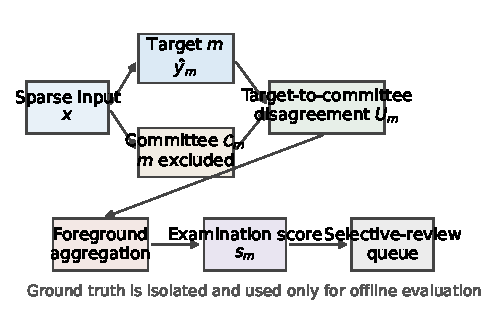
\includegraphics[width=\columnwidth]{figure_framework.pdf}
 \caption{Target-specific scoring and selective-review workflow. Ground truth is isolated from deployment scoring.}
 \label{fig:framework}
\end{figure}

\subsection{Failure boundary}
The decomposition
\begin{equation}
 \hat y_b=y+c+\epsilon_b
 \quad\Longrightarrow\quad
 \hat y_m-\hat y_b=\epsilon_m-\epsilon_b
 \label{eq:decomp}
\end{equation}
separates a shared systematic error $c$ from member-specific error $\epsilon_b$. Disagreement can expose target-specific deviations, but cancels an error common to all outputs. Diversity and non-perfectly-correlated errors are therefore necessary conditions. Consensus can falsely reassure when every interpolator removes the same structure, inherits the same training bias, or receives the same faulty preprocessing.

\subsection{Selective review}
Ground truth enters only offline. We define examination error $E_m$ as foreground MAE on generated slices. Examinations are sorted by increasing $s_m$; coverage $q$ is the retained, non-referred fraction. Risk $R(q)$ is mean $E_m$ among retained examinations. We report raw AURC, oracle and random AURC, and
\begin{equation}
 \mathrm{nAURC}=\frac{\mathrm{AURC}-\mathrm{AURC}_{\rm oracle}}
 {\mathrm{AURC}_{\rm random}-\mathrm{AURC}_{\rm oracle}},
\end{equation}
where zero is oracle and one is random ranking. Relative risk reduction is $\mathrm{RRR}(q)=[R_{\rm random}-R(q)]/R_{\rm random}$.

\section{Experiments}
\label{sec:experiments}

\textbf{Data and outputs.} We evaluate factor-four T2-weighted through-plane interpolation on IXI (115 examinations) \cite{ixi}, fastMRI-brain (24), and an internal NingXia cohort (22). NingXia predictions are held out across eight folds and pooled out of fold. IXI contains I$^3$Net, HAT, SwinIR, and ACSI outputs; the other cohorts contain the first three. Linear and cubic interpolation are available throughout. This gives ten fixed dataset--target profiles. No profile or examination is removed after observing its score.

\textbf{Integrity and sensitivity.} NIfTI case sets, duplicate identifiers, finite values, shapes, affines, orientations, and generated indices are checked before scoring. Stored neural outputs had been inversely mapped to source-volume intensity ranges, but model-specific clipping can still shift distributions. We therefore compare raw intensity with independent p1--p99, robust median/IQR, and min--max normalization. Masks include target thresholds 0.5--5\%, committee union/intersection/median, and one derived from observed anchors; a ground-truth mask is offline-only. These are retrospective sensitivities; the raw 1\% target mask remains pre-specified.

\textbf{Comparators.} Target-specific variants use mean, maximum, trimmed-mean, distance to the committee mean, and distance to its median image. Non-target-specific baselines use shared standard deviation and mean/median pairwise disagreement. Analytical baselines use linear/cubic residuals; gradient and Laplacian disagreement test structure-domain sensitivity. Every legal nonempty committee subset is recomputed from voxel outputs. SwinIR TTA is reported only as a local single-model comparison because it is unavailable on equal terms for all targets.

\textbf{Statistics.} Pixel Pearson correlation is computed within each examination foreground and aggregated with Fisher $z$; median/IQR and all-pixel values are secondary. Examination ranking uses Spearman $\rho$ and Kendall $\tau$. Selective review reports nAURC, RRR at 25/50/75\% retained coverage, and absolute retained MAE. We use 2,000 paired examination-bootstrap resamples with seed 20260715. Failure AUROC/AUPRC is secondary because the two smaller cohorts yield few top-decile positives.

\section{Results and Discussion}
\label{sec:results}

\begin{table*}[t]
 \centering
 \caption{Pre-specified all-member median disagreement. Pixel $r_z$ is the inverse Fisher-$z$ mean of per-examination foreground correlations. Coverage is the retained fraction; lower nAURC is better. MAE$_{50}$ remains dataset-scale dependent.}
 \label{tab:main}
 \resizebox{\textwidth}{!}{\begin{tabular}{llrrrrrr}
\toprule
Dataset & Target & $n$ & Pixel $r_z$ & Case $\rho$ [95\% CI] & nAURC [95\% CI] & RRR$_{50}$ & MAE$_{50}$ \\
\midrule
fastMRI-brain & HAT & 24 & 0.328 & 0.916 [0.758, 0.962] & 0.067 [0.017, 0.176] & 19.7\% & 69.47 \\
fastMRI-brain & I$^3$Net & 24 & 0.291 & 0.890 [0.713, 0.966] & 0.092 [0.029, 0.194] & 19.3\% & 55.96 \\
fastMRI-brain & SwinIR & 24 & 0.363 & 0.931 [0.781, 0.978] & 0.061 [0.012, 0.150] & 20.5\% & 70.23 \\
\midrule
IXI & ACSI & 115 & 0.435 & 0.954 [0.925, 0.972] & 0.035 [0.018, 0.060] & 50.1\% & 23.51 \\
IXI & HAT & 115 & 0.512 & 0.966 [0.940, 0.980] & 0.024 [0.012, 0.042] & 49.6\% & 24.72 \\
IXI & I$^3$Net & 115 & 0.351 & 0.951 [0.922, 0.969] & 0.044 [0.024, 0.073] & 52.1\% & 18.71 \\
IXI & SwinIR & 115 & 0.520 & 0.965 [0.937, 0.980] & 0.025 [0.012, 0.044] & 49.5\% & 24.92 \\
\midrule
NingXia & HAT & 22 & 0.277 & 0.929 [0.790, 0.975] & 0.076 [0.016, 0.228] & 22.2\% & 113.54 \\
NingXia & I$^3$Net & 22 & 0.356 & 0.914 [0.769, 0.970] & 0.063 [0.016, 0.186] & 23.1\% & 124.74 \\
NingXia & SwinIR & 22 & 0.279 & 0.936 [0.807, 0.983] & 0.036 [0.007, 0.120] & 21.4\% & 115.01 \\
\bottomrule
\end{tabular}
}
\end{table*}

\textbf{Error association and ranking.} Table~\ref{tab:main} reports every fixed profile. Spatial association is moderate (\PixelFisherRange), whereas examination ranking is strong (\CaseSpearmanRange). Aggregation can rank total error even when disagreement does not precisely localize each erroneous voxel. The smaller fastMRI-brain and NingXia cohorts have wider bootstrap uncertainty and do not support a clinical-safety claim.

\begin{figure*}[t]
 \centering
 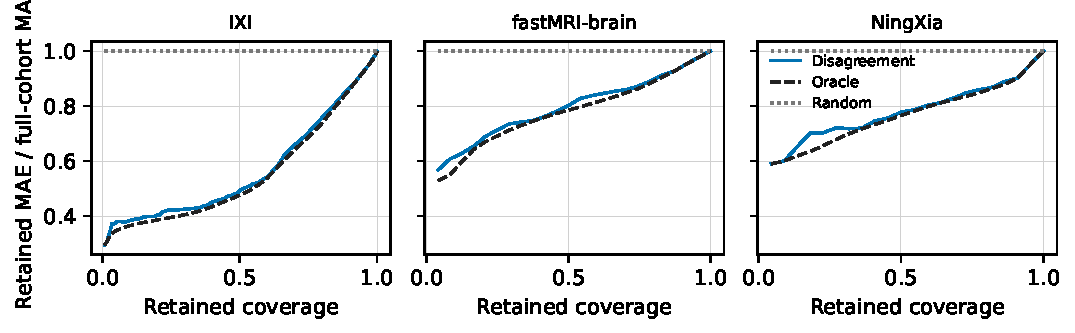
\includegraphics[width=0.68\textwidth]{figure_risk_coverage.pdf}\hfill
 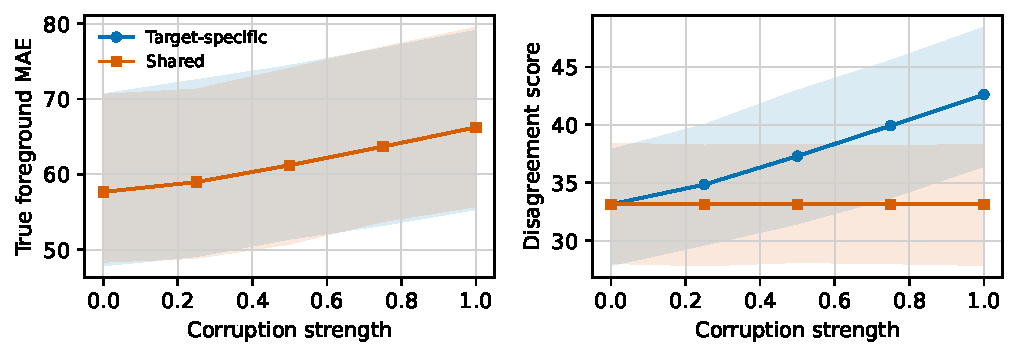
\includegraphics[width=0.29\textwidth]{shared_error_stress.pdf}
 \caption{Left: primary risk--coverage curves averaged over targets after normalization by full-cohort MAE. Right: target-specific versus shared additive-patch corruption over 20 fixed IXI examinations; bands are 95\% examination-bootstrap intervals.}
 \label{fig:risk}
\end{figure*}
\clearpage
\raggedbottom

\textbf{Selective review.} Across profiles, nAURC is \NAURCRange. At 50\% retained coverage, prioritizing the highest-score half for review lowers retained MAE by \RRRFiftyRange\ relative to random review (Fig.~\ref{fig:risk}). This supports ranking utility, not probability calibration.

\begin{table}[t]
 \centering
 \caption{Key ablations averaged over fixed target profiles. Score columns use the full committee; composition columns use all available members of each type. Lower nAURC is better.}
 \resizebox{\columnwidth}{!}{\begin{tabular}{lll}
\toprule
Dataset & Score nAURC: med./mean/std. & Committee nAURC: neural/analytic/full \\
\midrule
fastMRI-brain & 0.073/0.070/0.074 & 0.017/0.118/0.073 \\
IXI & 0.032/0.043/0.049 & 0.033/0.059/0.032 \\
NingXia & 0.058/0.056/0.033 & 0.094/0.031/0.058 \\
\bottomrule
\end{tabular}
}
 \label{tab:ablation}
\end{table}

\textbf{Composition and robustness.} Exact subset analysis is cohort dependent: neural-only subsets have mean nAURC 0.017 on fastMRI-brain and 0.029 for two peers on IXI, whereas analytical-only is strongest on NingXia (0.035). Thus no compact composition is universally reliable; the all-member committee remains the frozen default, not a retrospectively selected optimum. Median is also not uniquely best: mean, shared standard deviation, and pairwise mean have similar rankings, so our contribution is the target-specific protocol rather than a new elementary aggregator. Independently normalizing every output markedly degrades ranking, while input/committee masks largely preserve it.

\textbf{Alignment and mask sensitivity.} Raw source-intensity nAURC is 0.032/0.073/0.058 on IXI/fastMRI-brain/NingXia after averaging targets. Independently applying percentile, robust location--scale, or min--max normalization instead gives nAURC 0.322--1.391 and can reverse ranks; agreement in a common physical representation is therefore part of the method contract, not an optional cosmetic step. In contrast, input- and committee-derived masks have score-rank stability at least 0.973 across fixed profiles. Target-threshold sensitivity is concentrated on fastMRI-brain, where the 5\% mask reaches minimum stability 0.606. The offline ground-truth mask does not improve every cohort and is not used in deployment.

\textbf{Subset uncertainty.} Committee size alone is insufficient: over legal subsets, nAURC spans 0.009--0.139 on fastMRI-brain, 0.016--0.085 on IXI, and 0.022--0.122 on NingXia. The no-reference pairwise-output diversity proxy is only weakly associated with subset nAURC ($\rho=-0.141$ to 0.085), so it cannot select a compact committee reliably. These negative results motivate reporting the frozen full committee while exposing its online cost, rather than presenting an oracle-selected minimal subset.

At maximum synthetic strength, target MAE rose by \StressMaeIncrease. Disagreement rose by \StressTargetIncrease\ for target-specific corruption. Under shared corruption, target and mean committee MAE rose by \StressMaeIncrease\ and \StressCommitteeMaeIncrease, respectively, but disagreement changed by \StressSharedChange, directly illustrating Eq.~\eqref{eq:decomp}.

\textbf{Single-model comparator.} TTA gives $\rho=0.960$ and nAURC 0.023 versus 0.931 and 0.061 for the committee score, but weaker pixel association (0.306 versus 0.363). Its paired nAURC difference is $-0.038$ [95\% CI $-0.119$, 0.001], so the apparent gain is not conclusive. TTA is economical when only one model is available; cross-model scoring is attractive when deterministic peer outputs are already stored.

\textbf{Measured cost.} On 30 fixed examinations, a stored-output audit takes 1.18~s mean/2.87~s p95 on CPU, including 0.31~s NIfTI loading and 0.87~s scoring; mean input storage is 39.4~MiB and observed RSS peaks at 0.89~GiB. Linear/cubic interpolation alone takes 0.046/0.075~s. Online neural inference was not measured comparably and remains an additional cost.

\textbf{Review workflow.} A high $s_m$ prioritizes an examination for inspection; it does not prescribe discarding the reconstruction. A low score indicates consensus only within the available committee. This distinction is why continuous risk--coverage is primary, while top-decile failure AUROC/AUPRC is secondary and unstable with only three positive examinations per target in each smaller cohort.

\textbf{Limitations.} Equation~\eqref{eq:decomp} identifies the fundamental blind spot: shared blur, deletion, bias, or preprocessing errors can increase MAE without increasing disagreement. Highly correlated members reduce diversity; a correct but unusual detail can cause unnecessary referral. The intensity mask can omit tissue suppressed by the target and is not a clinical structure mask. The study is restricted to factor-four T2 brain MRI, has no reader study or downstream task, and MAE is not diagnostic harm. Thus $s_m$ is neither calibrated uncertainty nor evidence that agreement implies correctness.

\section{Conclusion}
Target-to-committee disagreement provides a ground-truth-free, target-specific reliability-ranking protocol for selective review of stored MRI interpolation outputs. It associates with examination error across three cohorts, but its performance depends on committee composition and diversity. It cannot identify errors shared by all members and should not be interpreted as a calibrated probability or clinical guarantee.

\clearpage
\section*{Compliance statement}
IXI and fastMRI are public research datasets. \textbf{Author confirmation required before submission:} state NingXia access, de-identification, and ethics approval or waiver identifiers, and insert the funding declaration. No clinical decision was made from the reported scores.

\bibliographystyle{IEEEbib}
\bibliography{references}

\end{document}
